\documentclass[11pt]{amsart}
\usepackage{geometry}                % See geometry.pdf to learn the layout options. There are lots.
\geometry{letterpaper}                   % ... or a4paper or a5paper or ... 
%\geometry{landscape}                % Activate for for rotated page geometry
%\usepackage[parfill]{parskip}    % Activate to begin paragraphs with an empty line rather than an indent
\usepackage{graphicx}
\graphicspath{ {images/} }
\usepackage{subfig}
\usepackage{amssymb}
\usepackage{epstopdf}
\DeclareGraphicsRule{.tif}{png}{.png}{`convert #1 `dirname #1`/`basename #1 .tif`.png}

\title{EM Algorithm}
\author{Elise McEllhiney}
\date{\today}                                           % Activate to display a given date or no date

\begin{document}
\maketitle

\section{Final Parameters}
\begin{align}
alpha & = [ 0.725 , 0.275 ] \\
mu & = [ 0.2877 , 4.2200 ] \\
sig & = [ [ 2.9346 , 0 ] , [ 2.7170 , 0 ] ] \\
muPrime & = [ 8.9707 ,  -0.4112 ] \\
sigPrime & = [ [ 2.7170 , 0 ] ,   [ 0, 1.7250 ] ]
\end{align}

\section{General Flow}
The main loop first executes the E-step which labels the points with their class guesses based on our "bad" starting parameters.  Then these labels are passed to the M-step which uses these labels to generate better mu and sigma values for the existing labels.  These new parameters are passed back to the E-step where the points are re-labelled and then passed to the M-step.  This loop continues until I either hit the maximum number of iterations(20) or it meets my convergence condition.

\section{Convergence Criterion}
I use a simple convergence criterions that checks if the new parameters a sufficiently different from the previous iterations parameters.  I do this by calculating the euclidean distance between the previous and existing mu coordinates.  As a double-check, I also generate a vector of my sigma values and do the same check.  If the distances between both old and new mu and the old and new sigmas is less than my epsilon value (.001), I consider the algorithm converged.  If either the mu or sigma values fail this check, then I don't consider it converged.

\begin{figure}
\caption*{Figures}
\begin{tabular}{cc}
\subfloat[iteration 1]{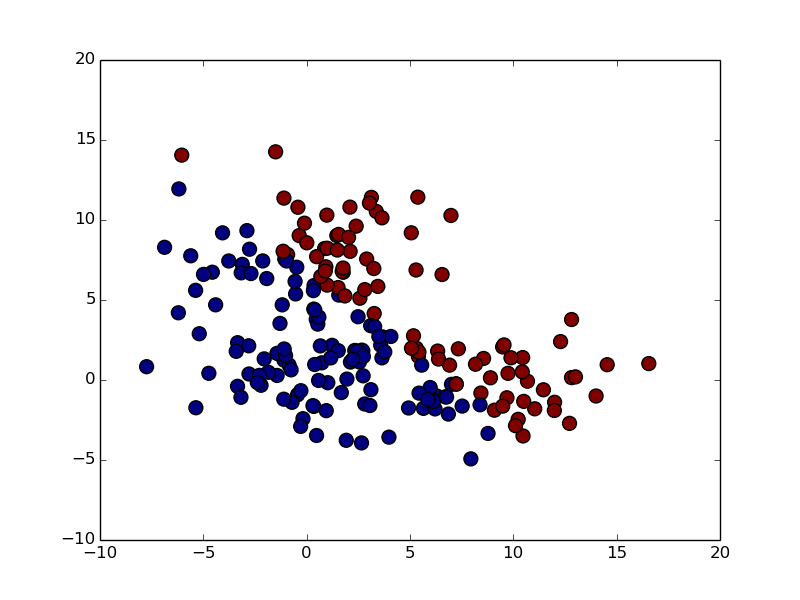
\includegraphics[width = 2in]{iter1}} &
\subfloat[iteration 2]{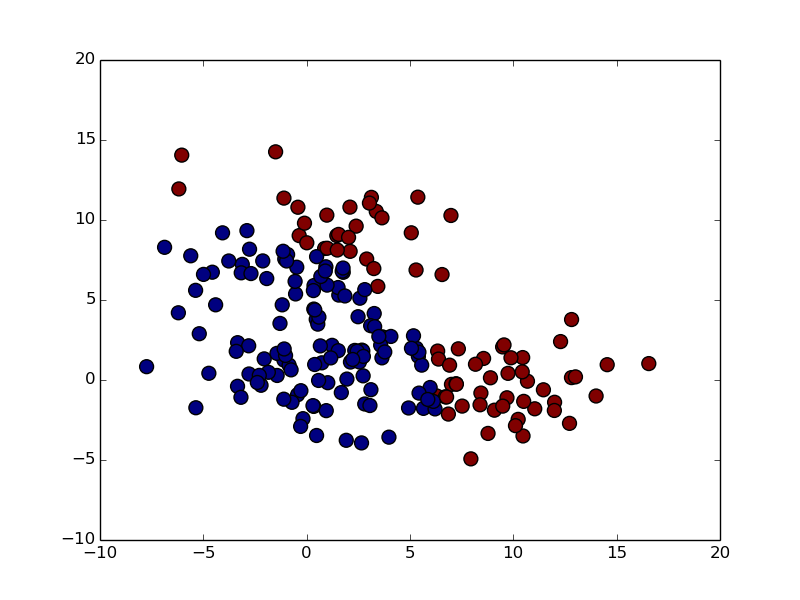
\includegraphics[width = 2in]{iter2}} \\
\subfloat[iteration 3]{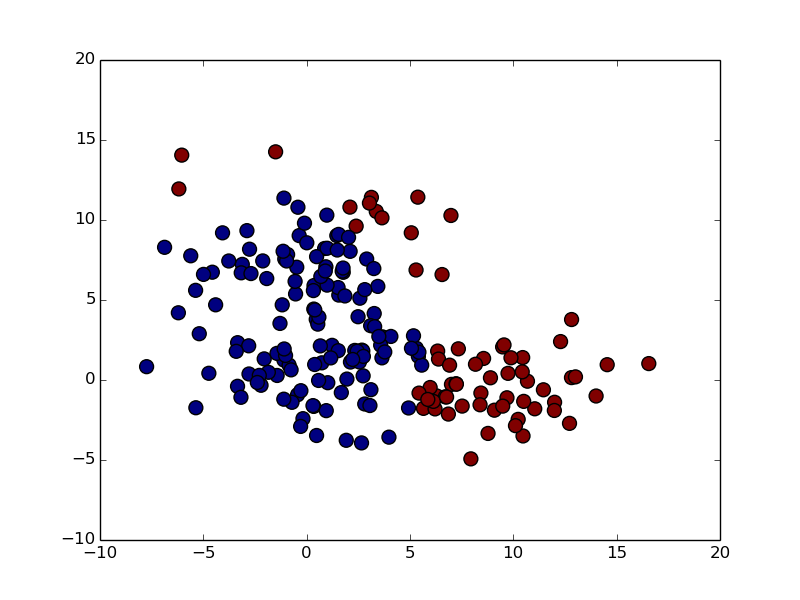
\includegraphics[width = 2in]{iter3}} &
\subfloat[iteration 4]{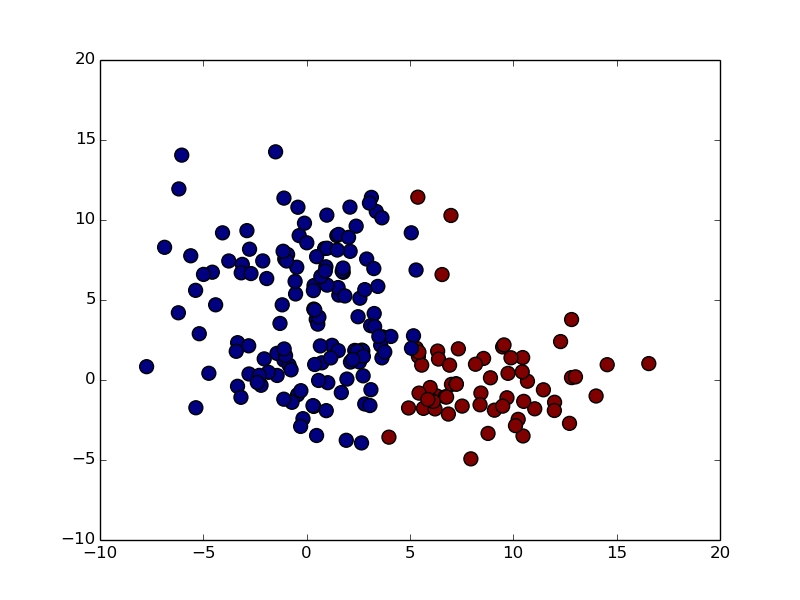
\includegraphics[width = 2in]{iter4}} \\
\subfloat[iteration 5]{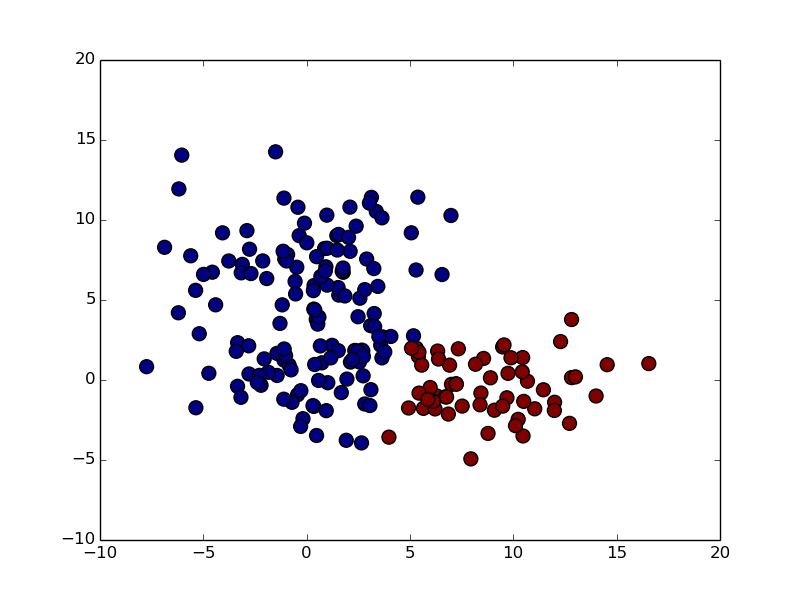
\includegraphics[width = 2in]{iter5}} &
\subfloat[iteration 6]{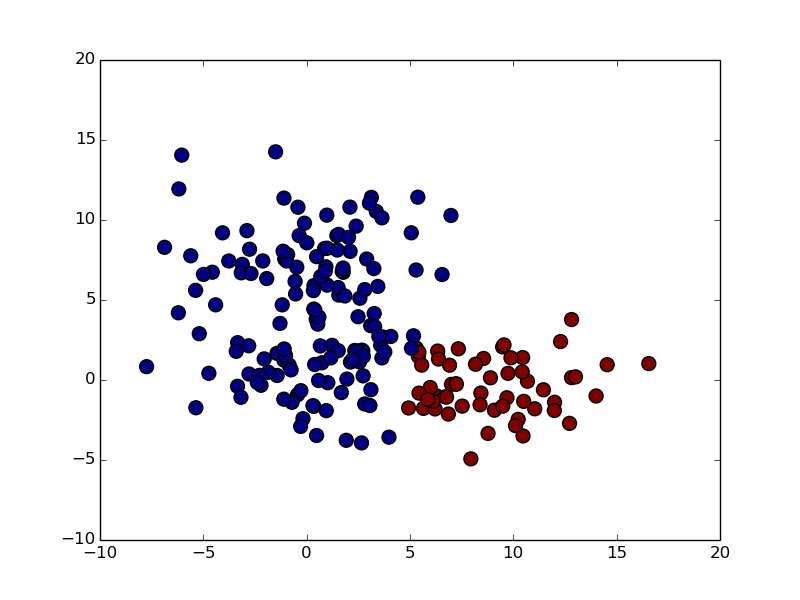
\includegraphics[width = 2in]{iter6}} \\
\subfloat[iteration 7]{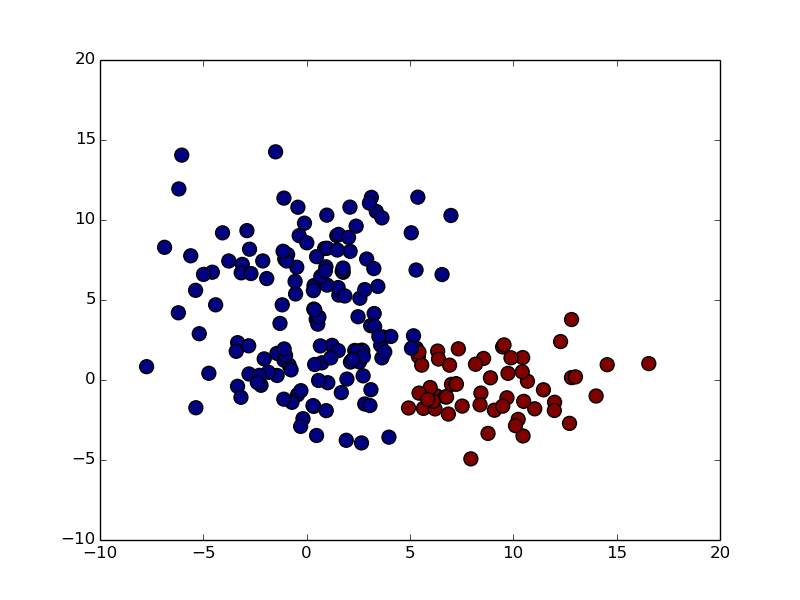
\includegraphics[width = 2in]{iter7}} &
\subfloat[iteration 8]{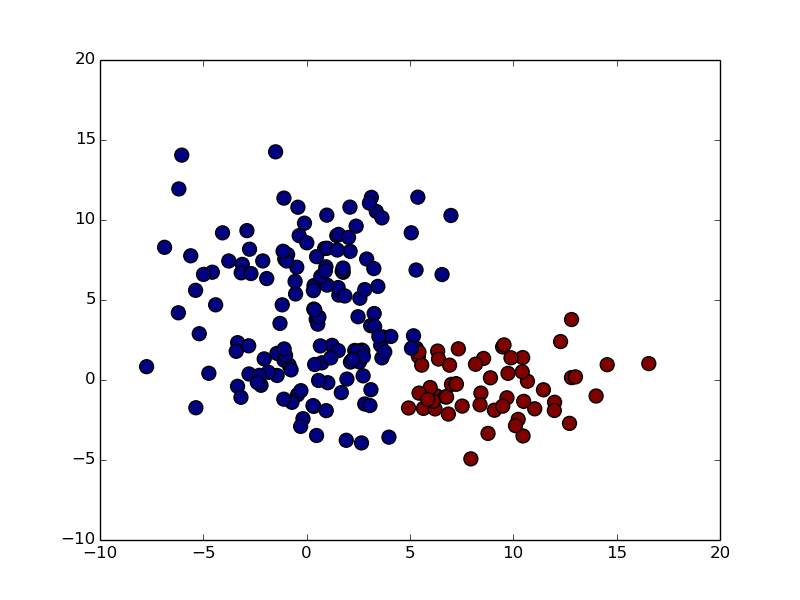
\includegraphics[width = 2in]{iter8}} \\
\end{tabular}
\end{figure}
\end{document}